\subsection{Hue intensity modulation based on rescaled ion counts}
\setcounter{step}{0}

\goldbox{}
\begin{minipage}[c]{0.6\textwidth}
Due to the statistical properties of the ion count data, ratio images may be noisy in areas where the ion counts of the denominator are low, possibly leading to distraction. Hue modulation intensity is designed to visually supress the noise and thus highlight the ratios in areas of interest. 
\end{minipage}\hfill
\begin{minipage}[c]{0.35\textwidth}
%\begin{center}
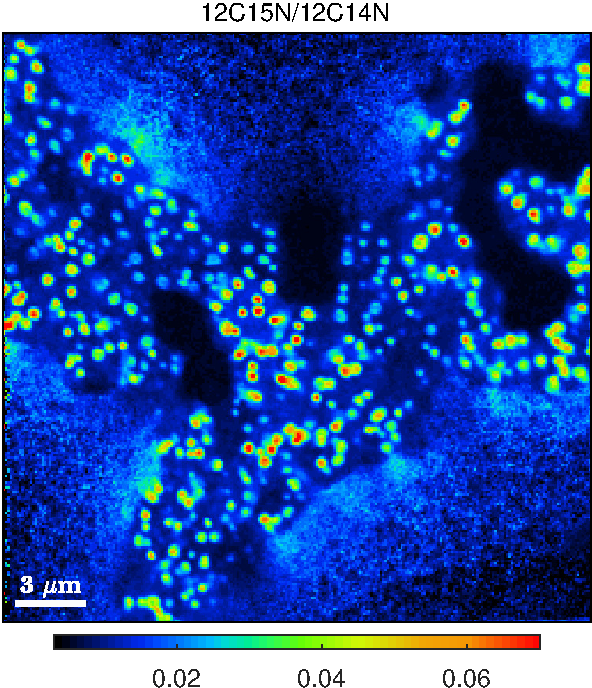
\includegraphics[width=2.3cm, valign=c]{figs6/12C15N-12C14N}
$\rightarrow$
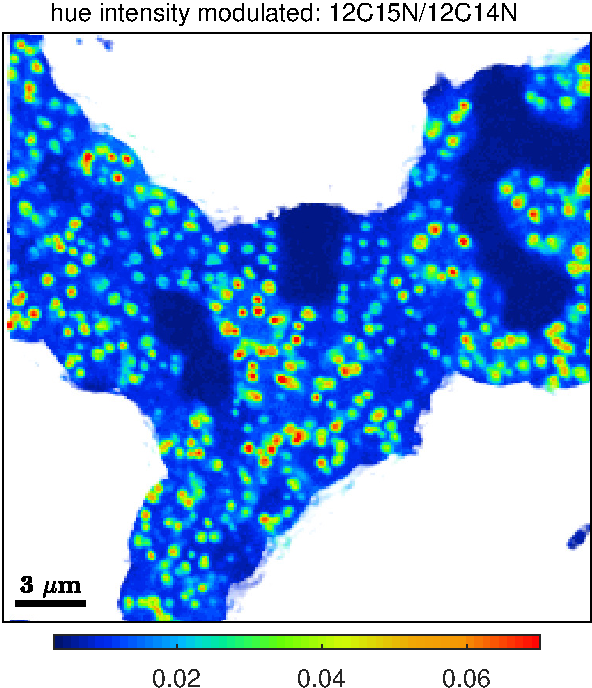
\includegraphics[width=2.3cm, valign=c]{figs6/12C15N-12C14Nc}
%\end{center}
\end{minipage}

\tcbe

For example, if \ttt{12C14N} and \ttt{12C15N} ions are detected from cells deposited on a~polycarbonate filter, the ion counts will be high in areas corresponding to cells but very low in areas corresponding to the filter (Fig.~\ref{fig:hue}A--B). As a~result, the ratio image \ttt{12C15N/12C14N} will be noisy in areas on the filter, distracting the perception of the variation in the \ttt{15N/14N} ratio within cells (Fig.~\ref{fig:hue}C). 

\begin{figure}[!ht]
\centering
\begin{tabular}{ccc}
(A) & (B) & (C) \\
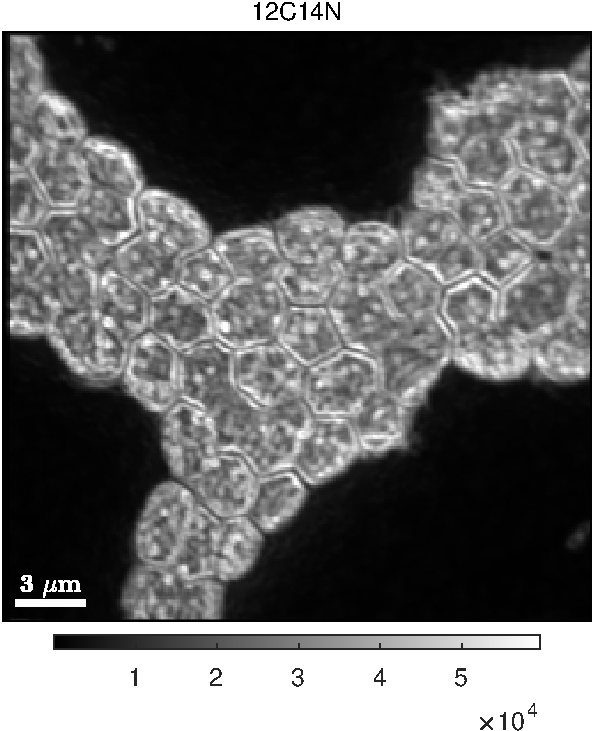
\includegraphics[scale=0.4, valign=t]{figs6/12C14N}
&
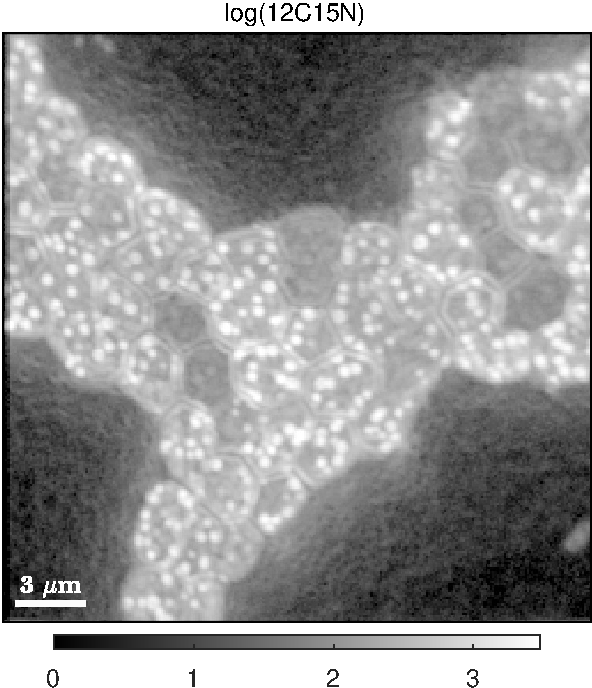
\includegraphics[scale=0.4, valign=t]{figs6/12C15N}
&
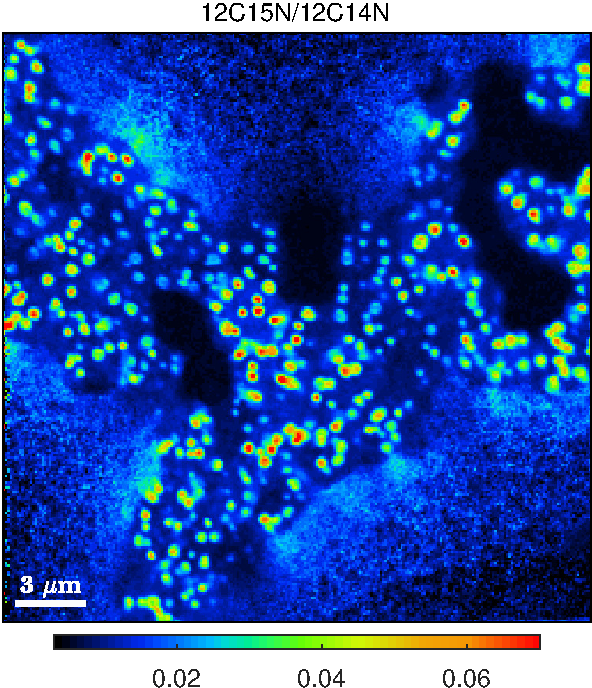
\includegraphics[scale=0.4, valign=t]{figs6/12C15N-12C14N}
\\
(D) & (E) & (F) \\
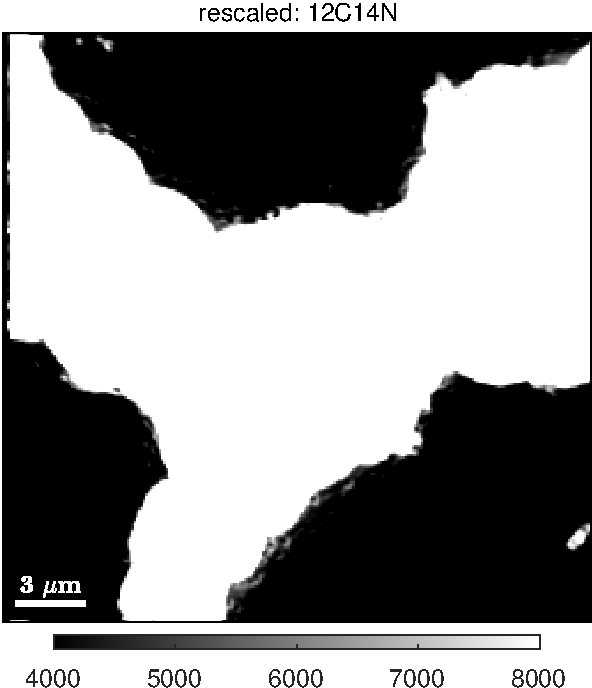
\includegraphics[scale=0.4, valign=t]{figs6/12C14Nb}
&
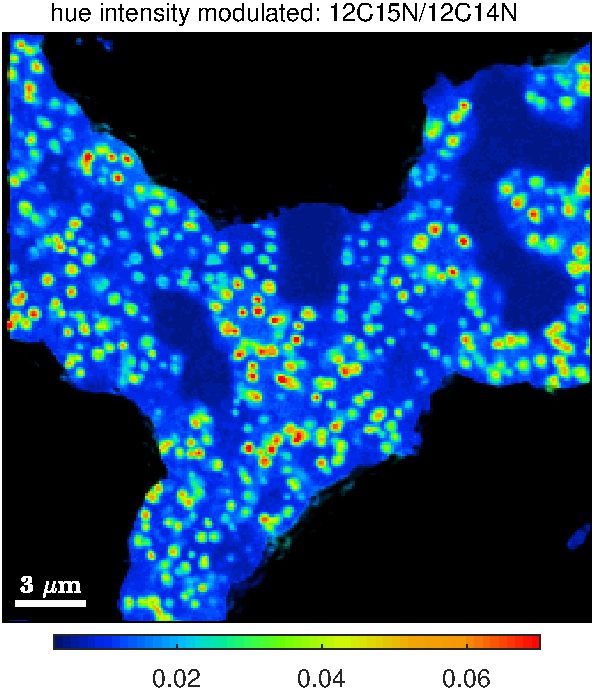
\includegraphics[scale=0.4, valign=t]{figs6/12C15N-12C14Nb}
&
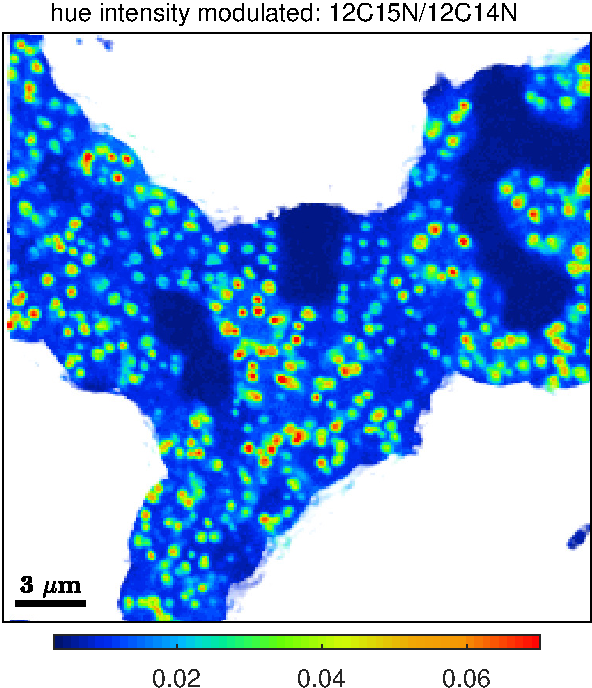
\includegraphics[scale=0.4, valign=t]{figs6/12C15N-12C14Nc}
\end{tabular}
\caption{\label{fig:hue}%
Manipulation of the image appearance by hue intensity modulation. (A) \ttt{12C14N} ion counts, shown in the linear scale. Note the large contrast between the counts from areas with cells and areas on the filter. (B) \ttt{12C15N} ion counts, shown in the logarithmic scale. (C) \ttt{12C15N/12C14N} ratio image. Note the noise in areas on the filter. (D) The same \ttt{12C14N} ion count image as in panel~A, but rescaled such that the areas with and without cells appear white and black, respectively. (E--F) The same \ttt{12C15N/12C14N} ratio image as in panel~C, but with hue intensity modulation applied based on the image in panel~D. The areas on the filter can be shown in black (E) or white (F).}
\end{figure}

Use the following steps to manipulate the ratio image such that the noise perception from areas on the filter will be minimized, as illustrated in Fig.~\ref{fig:hue}E--F.

\s{In the main LANS window, rescale the \ttt{12C14N} image (i.e., the mass that defines the cells) such that the cells will appear white and the filter will appear black (Fig.~\ref{fig:hue}D).}

\s{Select the \lanscb{Modulate hue intensity} checkbox and add number~4 in the \lanstf{mass} field next to it.}

\nbx{In this example, number 4 is chosen because for this particular dataset, the identifier of the \ttt{12C14N} mass is~4.}

\s{Select \lans{Output} $\ra$ \lans{Display ratios} to re-export the \ttt{12C15N/12C14N} ratio image.}

\nbx{The modified image will look as shown in Fig.~\ref{fig:hue}E, with areas on the filter being so dark (black) that the distracting noise is virtually invisible.}

\nnb{You can modify this behaviour by changing the dark areas to bright (white) areas, as explained in the next steps.}

\s{Select \lans{Preferences} $\ra$ \lans{Additional output options}, and in the window that opens, select the \lanscb{Use white to modulate hue} checkbox and click \lans{Apply}. }

\s{Then, back in the main LANS window, change the \lanstf{color} next to the \lanscb{Include ROIs outline} checkbox to \ttt{k} (corresponding to black).}

\nbx{This will ensure that the scale bar will be visible in the exported image (i.e., displayed in black rather than white).}

\s{Re-export the ratio image by selecting \lans{Output} $\ra$ \lans{Display ratios}.}

\nbx{The modified image will look as shown in Fig.~\ref{fig:hue}F, with areas on the filter being so bright (white) that the distracting noise is virtually invisible.}

\vskip1mm\noindent
We emphasize that hue intensity modulation is a~powerful feature and should be used \bb{responsibly}. It may be used to supress distracting but irrelevant information, such as in the example above, but \bb{not} hide distracting but possibly important information in the image.
